%%%%%%%%%%%%%%%%%%%%%%%%%%%%%%%%%%%%%%%%%
% Structured General Purpose Assignment
% LaTeX Template
%
% This template has been downloaded from:
% http://www.latextemplates.com
%
% Original author:
% Ted Pavlic (http://www.tedpavlic.com)
%
% Note:
% The \lipsum[#] commands throughout this template generate dummy text
% to fill the template out. These commands should all be removed when 
% writing assignment content.
%
%%%%%%%%%%%%%%%%%%%%%%%%%%%%%%%%%%%%%%%%%

%%%%%%%%%%%%%%%%%%%%%%%%%%%%%%%%%%%%%%%%%
%TODO
%
% BLACK BOX SEQUENCE DIAGRAMMEN
% MORPHOLOGISCH ONDERZOEK
% WHITE BOX OMSCHRIJVING
% 
%%%%%%%%%%%%%%%%%%%%%%%%%%%%%%%%%%%%%%%%%

%----------------------------------------------------------------------------------------
%	PACKAGES AND OTHER DOCUMENT CONFIGURATIONS
%----------------------------------------------------------------------------------------
\documentclass[12pt]{article} % Default font size is 12pt, it can be changed here
\usepackage[dutch]{babel}
\newcommand{\sectionbreak}{\clearpage} % Starts every section on its own page
\usepackage[table,xcdraw]{xcolor}
\usepackage{geometry} % Required to change the page size to A4
\geometry{a4paper} % Set the page size to be A4 as opposed to the default US Letter
\usepackage{fancyhdr} % Required for custom headers
\usepackage{extramarks} % Required for headers and footers
\usepackage{lastpage} % Required to determine the last page for the footer
\usepackage{graphicx} % Required for including pictures
\usepackage{multirow} % Required for table
\usepackage{float} % Allows putting an [H] in \begin{figure} to specify the exact location of the figure
\usepackage{wrapfig} % Allows in-line images such as the example fish picture
\usepackage{lipsum} % Used for inserting dummy 'Lorem ipsum' text into the template
\usepackage{booktabs} % used for table?
\usepackage{pdflscape}
\usepackage{booktabs} % used for table
\linespread{1.2} % Line spacing

\graphicspath{{imgs/}}
%----------------------------------------------------------------------------------------
%	HEADER/FOOTER
%----------------------------------------------------------------------------------------


\pagestyle{fancy}
\lhead{Julian \textsc{West} \& Jelle Braat} % Top left header
\rhead{ Robochallenge robot} % Top center header
\lfoot{\lastxmark} % Bottom left footer
\cfoot{} % Bottom center footer
\rfoot{Pagina\ \thepage\ van de\ \pageref{LastPage}} % Bottom right footer
\renewcommand\headrulewidth{0.4pt} % Size of the header rule
\renewcommand\footrulewidth{0.4pt} % Size of the footer rule

\setlength\parindent{0pt} % Removes all indentation from paragraphs

%----------------------------------------------------------------------------------------
%	TITLE PAGE
%----------------------------------------------------------------------------------------
\begin{document}

\begin{titlepage}
\pagenumbering{Roman}
\newcommand{\HRule}{\rule{\linewidth}{0.5mm}} % Defines a new command for the horizontal lines, change thickness here

\center % Center everything on the page

\includegraphics[scale=.1,keepaspectratio]{avans.pdf} \\
\textsc{\Large Avans Hogeschool Breda}\\[0.5cm] % Major heading such as course name
\textsc{\large Real-Time Systems (RTSYS)}\\[0.5cm] % Minor heading such as course title
\HRule \\[0.4cm]
{ \huge \bfseries Robochallenge Robot Design Document}\\[0.4cm] % Title of your document
\HRule \\[1.5cm]

\begin{minipage}{0.4\textwidth}
\begin{flushleft} \large
\emph{Auteurs:}\\
Julian \textsc{West} \\
Jelle \textsc{Braat} \\
\end{flushleft}
\end{minipage}
~
\begin{minipage}{0.4\textwidth}
\begin{flushright} \large
\emph{Leraren:} \\
Joli \textsc{van Kruijsdijk} \\ % Supervisor's Name
Hans \textsc{van der Linden} \\
Paul \textsc{Lindelauf} %Indien Paul overneemt op 09/02
%Jan \textsc{Oostindie} %Onbekend of hij wel meehelpt
\end{flushright}
\end{minipage}\\[4cm]

{\large \today}\\[3cm] % Date, change the \today to a set date if you want to be precise
Versie: 0.1
\vfill % Fill the rest of the page with whitespace

\end{titlepage}

%----------------------------------------------------------------------------------------
%	TABLE OF CONTENTS
%----------------------------------------------------------------------------------------
%\setcounter{tocdepth}{1} % Uncomment this line if you don't want subsections listed in the ToC
\tableofcontents
\newpage
\pagenumbering{arabic}
\clearpage
%----------------------------------------------------------------------------------------
% Introduction
%----------------------------------------------------------------------------------------
\section{Introductie}
\label{sec:introduction}
\lipsum[0-3]
\newpage
%----------------------------------------------------------------------------------------
% Requirements
%----------------------------------------------------------------------------------------
%Funcitonele
%Operationele
%QoS(quality of service)
%Parametrische
%Design

\section{Eisen}
\label{sec:requirements}
In dit hoofdstuk worden eisen gesteld aan het systeem van de Robochallenge robot. Deze eisen zijn onderverdeeld in de volgende 5 typen eisen. Ten eerste de functionele eisen, daarna operationele, gevolgd door Quality of Service(QoS) eisen, hierna de parametrische eisen en als laatste de design eisen. Sommige eisen kunnen verder worden gegroepeerd met gerelateerde eisen.\\
Met de operationele eisen wordt bedoeld hoe het systeem met de diverse elementen in de omgeving zal samenwerken. 
Onder de functionele eisen wordt het gedrag en het kunnen van het systeem verstaan.
QoS eisen houdt in hoe goed het systeem zijn operationele en functionele eisen uitvoert.
Parametrische eisen betekent eisen aan de grootte van het fysieke systeem. 
Ten slotte valt onder design eisen de eisen aan de impressie en bruikbaarheid van het systeem.

\subsection{Operationele eisen}

\newcommand\litem[1]{\item{\bfseries #1\\}}
\begin{enumerate}
\litem{Grijpen} De robot moet een bal kunnen kunnen grijpen.
\litem{Plaats 1} De robot moet zijn plaats in een ruimte kunnen detecteren.
\litem{Plaats 2} De robot moet de limieten (muren) van een ruimte kunnen bepalen.
\litem{Starten} De robot moet gestart worden door een enkele startknop.
\litem{Noodknop} De robot moet voorzien zijn van een noodknop die onmiddellijk alle functionaliteiten van de robot stop legt.
\litem{Aandrijving} De robot mag alleen elektrisch aangedreven worden.
\litem{Pitstop} De robot moet naar de pitstop kunnen navigeren.
\litem{Instellen} De robot moet vanaf een kaart een keuze maken m.b.t. ballen keuze.
\litem{Geluid} De robot moet een zoemer hebben voor feedback aan de gebruiker.
\end{enumerate}

\subsection{Functionele eisen}
\begin{enumerate}
\litem{Kalibreren} De robot moet op basis van input zijn onderdelen automatisch kunnen bij- of instellen.
\litem{Bewegen} De robot moet autonoom bewegen, dus zonder enige ingrijpen van een persoon.
\litem{Opslaan} De robot moet de ballen naar een intern reservoir kunnen brengen.
\litem{Objecten} De robot moet de anderskleurige ballen vinden in relatie met zijn positie.
\litem{Kleur} De robot moet distinctie kunnen brengen in de kleuren van de ballen. 
\litem{Keuze} De robot moet de correcte bal pakken die de missie vereist.
\litem{Muren} De robot moet wanneer deze tegen een muur aanrijdt kiezen om een andere kant op te gaan.
\litem{Programmeren} De robot moet kunnen worden geherprogrammeerd van een computer via USB.  
\end{enumerate}
\newpage

\subsection{Quality of Service eisen}
\begin{enumerate}
\litem{Flexibility 1} De robot moet kunnen bewegen in 8 assen van vrijheid (Vooruit, achteruit, links, rechts en diagonaal).
\litem{Flexibility 2} De robot moet een bal kunnen grijpen vanaf diverse invalshoeken.
\litem{Flexibility 3} De robot moet een bal kunnen grijpen op diverse hoogten.
\litem{Stability} De robot mag ballen die zijn gegrepen niet laten vallen.
\litem{Reliability} De robot moet ballen kunnen onderscheiden in hun primaire of secundaire kleur.
\end{enumerate}

\subsection{Parametrische eisen}
\begin{enumerate}
\litem{Opslag} De robot moet een opslag hebben die voldoende groot is voor 17 ballen met een diameter van 7cm.
\litem{Grootte} De robot mag niet groter zijn dan 50x40cm.
\litem{Verplaatsbaar} De robot zou handmatig te verplaatsen moeten zijn. 
\litem{Stroomtoevoer} De robot moet voorzien zijn van zijn eigen stroom toevoer.
\litem{Spanning} De maximale interne spanning binnen de robot is 48 volt.
\litem{Toegankelijkheid} Onderdelen moeten toegankelijk zijn om tussen missies aanpassingen te kunnen maken.

\end{enumerate}
\newpage

\subsection{Design eisen}
\begin{enumerate}
\litem{Licht} De robot mag geen verblindend licht gebruiken.
\litem{Misleiden} De robot mag niet voorzien zijn van onderdelen die de tegenstander kan misleiden.
\litem{Offensief} De robot mag niet voorzien zijn van offensieve middelen zoals rookbommen, stroomstoten of Elektromagnetische Pulse(EMP) wapens.
\litem{Noodknop} De noodknop op de robot moet zichtbaar en toegankelijk zijn.
\end{enumerate}
\newpage

%----------------------------------------------------------------------------------------
% Use Case
%----------------------------------------------------------------------------------------
\section{Use case beschrijvingen}
Dit hoofdstuk is toegewijd aan het omschrijven van de gebruikers interactie met het systeem. Elke use case beschrijft hoe een gebruiker een functie van het systeem uitvoert en hoe het systeem (visueel) hierop reageert.

\subsection{Use case diagram}

Het volgende diagram laat schematisch zien welke operaties een gebruiker kan uitvoeren met het systeem. Elke use case statement is als een eis te herleiden naar een van de eisen.
\begin{center}
\begin{figure}
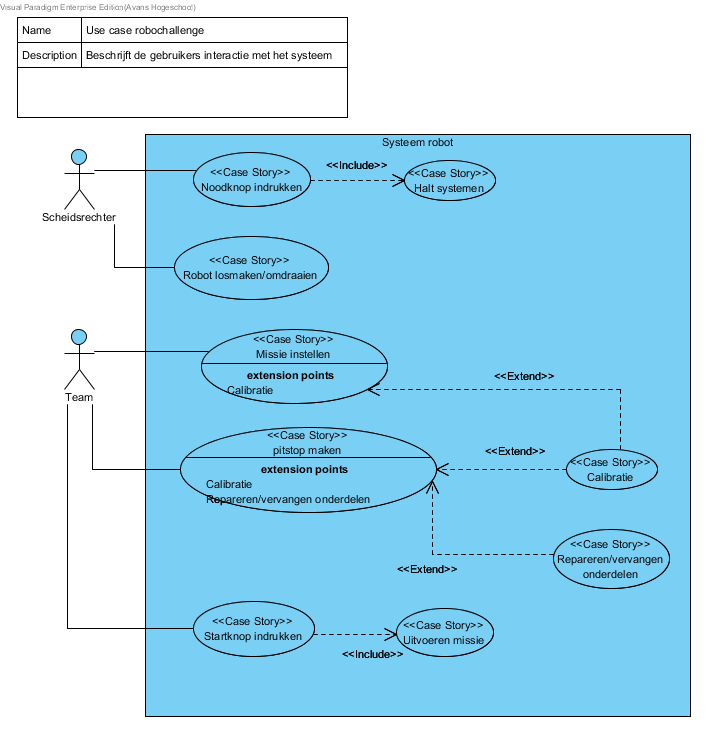
\includegraphics[scale=.9]{usecase.png}
\caption{Use case diagram van het globale systeem}
\label{fig:usecase}
\end{figure}
\end{center}
\clearpage
\newpage

\subsection{Use case omschrijvingen}

\begin{center}
\begin{figure}[H]
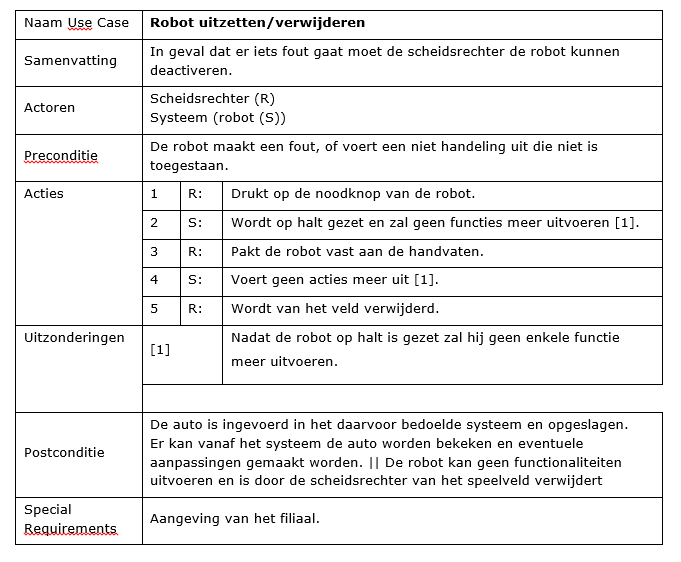
\includegraphics[scale=.9]{uc1.png}
\caption{Use case diagram van het globale systeem}
\label{fig:usecase}
\end{figure}
\end{center}

\begin{center}
\begin{figure}
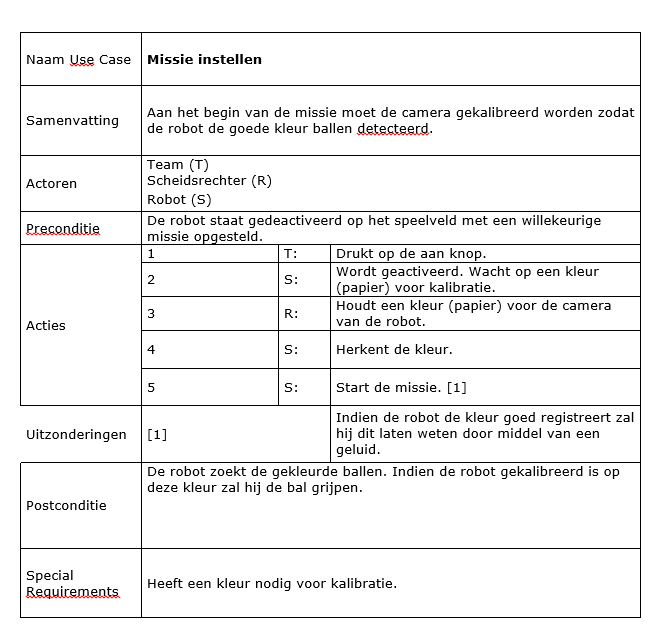
\includegraphics[scale=.9]{uc2.png}
\caption{Use case omschrijving}
\label{fig:usecase}
\end{figure}
\end{center}

\begin{center}
\begin{figure}
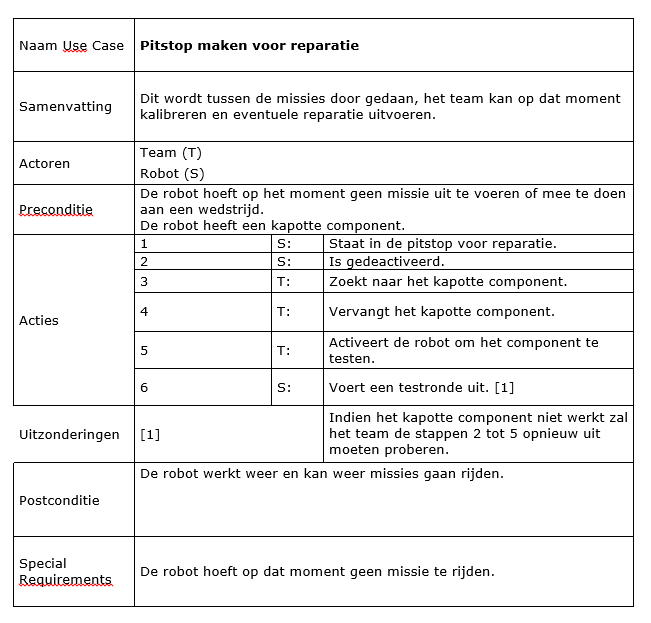
\includegraphics[scale=.9]{uc3.png}
\caption{Use case omschrijving}
\label{fig:usecase}
\end{figure}
\end{center}

\begin{center}
\begin{figure}
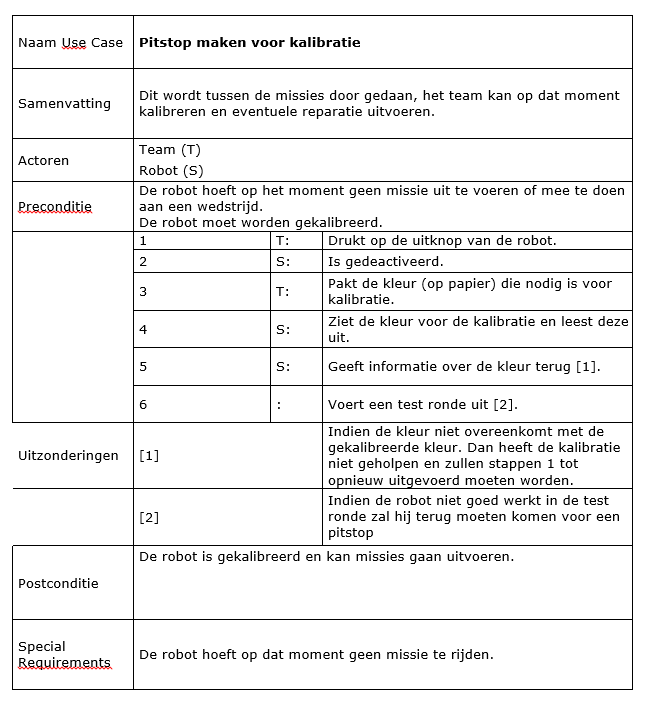
\includegraphics[scale=.9]{uc4.png}
\caption{Use case omschrijving}
\label{fig:usecase}
\end{figure}
\end{center}

\newpage
%----------------------------------------------------------------------------------------
% Black box subsysteem architectuur
%----------------------------------------------------------------------------------------
\section{Black box subsysteem architectuur}
\label{sec:Black box subsysteem architectuur}
Een black box subsysteem is een gesloten decompositie van het systeem. Dit houdt in dat een black box subsysteem een globaal overzicht is wat het systeem bevat, aan hardware componenten en wat deze hardware componenten kunnen uitvoeren.

\subsection{Interfaces}
\begin{itemize}
\item Het systeem heeft logica nodig om te functioneren. Dit is het belangrijkste component van het systeem en zal de alle (volgende) onderdelen combineren.
\item Het systeem heeft vermogen nodig om te kunnen functioneren, dit vermogen moet gestuurd kunnen worden naar de juiste componenten.
\item Het systeem maakt gebruik van vision, dit is een camera. De camera detecteert en registreert zijn omgeving.
\item Het systeem heeft aandrijving nodig voor verplaatsing over het speelveld, dit houdt ook in dat het systeem kan draaien.
\item Het systeem heeft een grijper. De grijper moet ballen van het speelveld grijpen en verplaatsen naar het reservoir.
\item Het systeem heeft input en output (I/O) nodig. Dit zijn verschillende hardware componenten waar het systeem gebruik van zal maken. I/O is een verzamel naam voor alle overige componenten. 
\end{itemize}
\clearpage

\subsection{Structured classes}
\begin{center}
\begin{figure}[h]
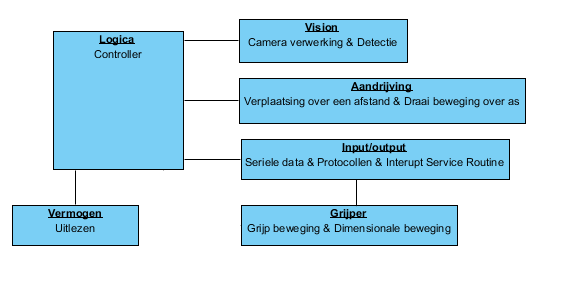
\includegraphics[scale=1.]{BlackBoxDiagram.png}
\caption{Black box subsysteem diagram}
\label{fig:deployment}
\end{figure}
\end{center}
\clearpage
\subsection{Sequence/State Machine diagram}

\newpage%----------------------------------------------------------------------------------------
% Deployment view
%----------------------------------------------------------------------------------------
\section{Deployment view}
\label{sec:Deployment view}
Een deployment view beschrijft de interne omgeving waar het systeem op draait. Indien de interne omgeving ook externe afhankelijkheden heeft dan worden deze ook beschreven in het systeem. Alles zal dus op runtime van het systeem draaien ook de externe afhankelijkheden.

\subsection{Morfologisch overzicht}
Het morfologische overzicht is een vergelijking tussen componenten . Deze componenten zijn onder anderen aandrijving en grijpen. Er wordt een vergelijking gemaakt, met de componenten, die de voordelen en nadelen bepaald van componenten die gebruikt kunnen worden in het systeem.

\subsubsection{Beweging(Aandrijving)}
\begin{center}
\begin{figure}[h]
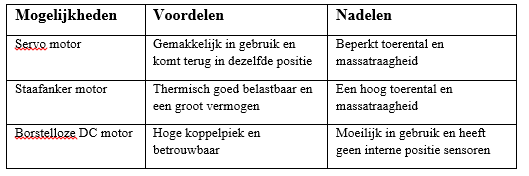
\includegraphics[scale=1.]{tabelAand.png}
\caption{tabel aandrijving}
\label{fig:deployment}
\end{figure}
\end{center}
\clearpage

\subsubsection{Oppakken (Grijpen)}
\begin{center}
\begin{figure}[h]
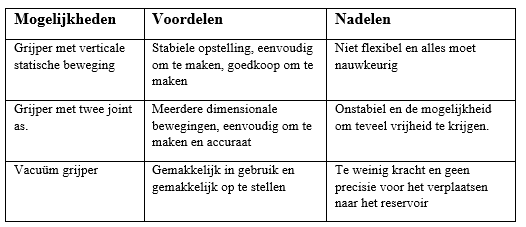
\includegraphics[scale=1.]{tabelOppakken.png}
\caption{tabel oppakken}
\label{fig:deployment}
\end{figure}
\end{center}


\subsubsection{Zoomer (I/O)}
\begin{center}
\begin{figure}[h]
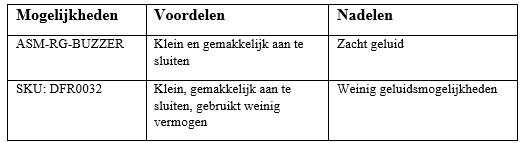
\includegraphics[scale=1.]{tabelZoomer.png}
\caption{tabel zoomer}
\label{fig:deployment}
\end{figure}
\end{center}
\clearpage

\subsubsection{Knop (I/O)}
\begin{center}
\begin{figure}[h]
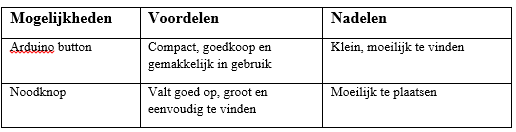
\includegraphics[scale=1.]{tabelKnop.png}
\caption{tabel knoppen}
\label{fig:deployment}
\end{figure}
\end{center}

\subsubsection{Camera (Vision)}
\begin{center}
\begin{figure}[h]
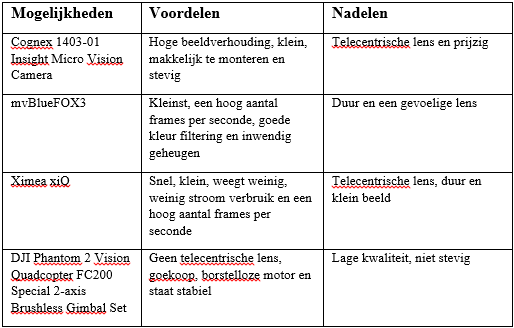
\includegraphics[scale=1.]{tabelCam.png}
\caption{tabel aandrijving}
\label{fig:deployment}
\end{figure}
\end{center}
\clearpage

\subsubsection{Batterij (Vermogen)}
\begin{center}
\begin{figure}[h]
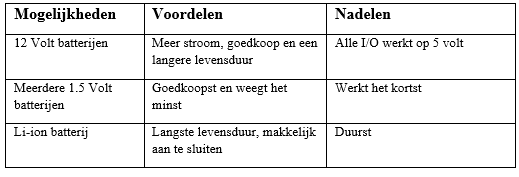
\includegraphics[scale=1.]{tabelBat.png}
\caption{tabel aandrijving}
\label{fig:deployment}
\end{figure}
\end{center}
\clearpage

\subsection{Deployment diagram}
\begin{center}
\begin{figure}[h]
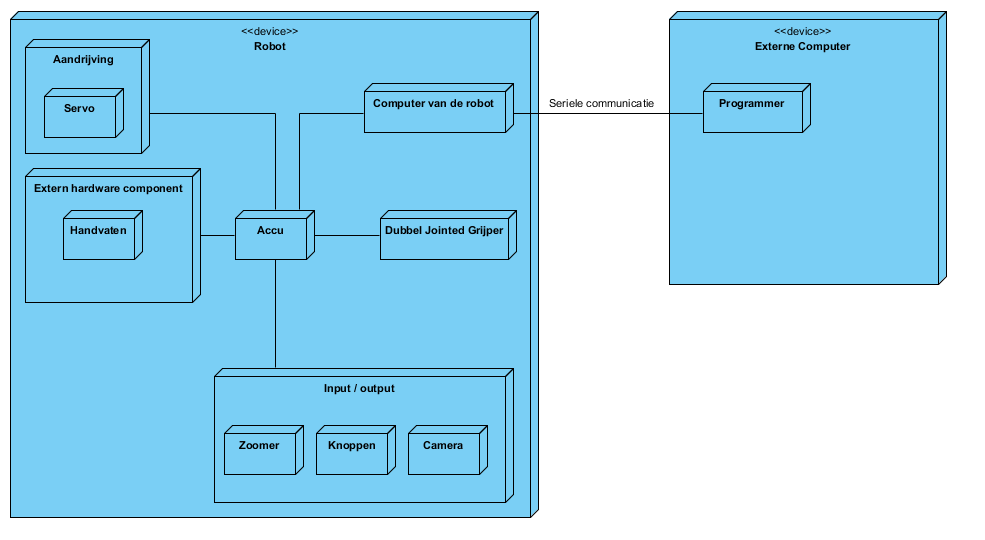
\includegraphics[scale=.65]{deployment.png}
\caption{Deployment view diagram van de robot}
\label{fig:deployment}
\end{figure}
\end{center}
\clearpage
\newpage%----------------------------------------------------------------------------------------
% White box subsysteem architectuur
%----------------------------------------------------------------------------------------
\section{White box subsysteem architectuur}
\label{sec:conclusion}

\subsection{Interfaces}
\subsubsection{Logica}
De logica stuurt alle data door en verwerkt data. Dit gaat door middel van een controller. De controller ontvangt de data, daarna wordt er bepaald wat er met de data moet gebeuren en hoe waar het naartoe gestuurd moet worden. Dit is het hart van het systeem.
\subsubsection{Aandrijving}
De motor is een servo die op verschillende manieren data kan gebruiken. De motor bestaat uit verschillende onderdelen die verschillende mogelijkheden hebben:
\begin{itemize}
\item PWM - dit is de Pulse-width modulation
\item Rijden -
\item Noodstop - 
\end{itemize}
\subsubsection{Grijper}
\subsubsection{Input/Output}
\subsubsection{Vision}
\subsubsection{Vermogen}

\begin{itemize}
\item Het systeem heeft logica nodig om te functioneren. Dit is het belangrijkste component van het systeem en zal de alle (volgende) onderdelen combineren.
\end{itemize}

\subsection{Structured classes}
\begin{center}
\begin{figure}[h]
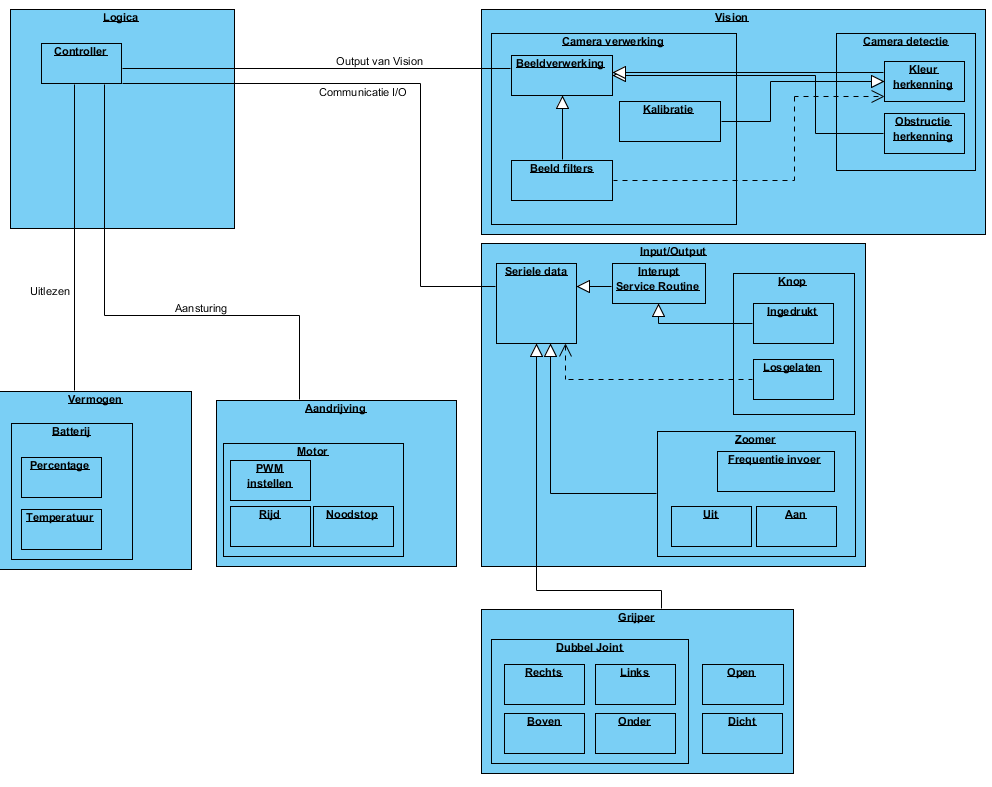
\includegraphics[scale=.6]{WhiteBoxDiagram.png}
\caption{White box diagram}
\label{fig:deployment}
\end{figure}
\end{center}
\clearpage
\newpage

\subsection{Sequence/State Machine diagram}

\newpage%----------------------------------------------------------------------------------------
%	Glossary
%----------------------------------------------------------------------------------------
%\clearpage
%\printglossaries
%----------------------------------------------------------------------------------------
%	Bibliography
%----------------------------------------------------------------------------------------
% \clearpage
% \bibliographystyle{plainurl}
% \nocite{*}
% \bibliography{Bibliography}
%----------------------------------------------------------------------------------------
%	Appendix
%----------------------------------------------------------------------------------------
%\addcontentsline{toc}{section}{Appendix A - Interns' hip assignment}
%\includepdf[pagecommand=\section*{Appendices}\subsection*{Appendix A - Internship assignment} The document including the assignment to the interns from Streamit,pages=-,scale=0.67]{appendices/Internship_assignments.pdf}
%----------------------------------------------------------------------------------------
%	End of document
%----------------------------------------------------------------------------------------
\end{document}

%figure example
%figures~\ref{fig:ganttFig1} and~\ref{fig:ganttFig2}.\\
%\begin{figure}
%\includegraphics{gantt4_2.png}
%\caption{Iterations of the project}
%\label{fig:ganttFig1}
%\end{figure}
%\begin{figure}
%\begin{center}
%%\includegraphics[angle=90,width=\textwidth,height=\textheight,keepaspectratio]{versie4.png}
%\includegraphics[angle=90,width=\textwidth,height=\textheight,keepaspectratio]{gantt4.png}
%\caption{Gantt chart of the planning}
%\label{fig:ganttFig2}
%\end{center}
%\end{figure}